\documentclass[12pt,a4paper]{report}
\usepackage{verbatim}
\usepackage{alltt}
\usepackage{graphicx}
\usepackage[latin1]{inputenc}
%\usepackage[norsk]{babel}

\begin{document}
\title{User Manual}


\section*{Foreword}
This document is part of a bachelor project developed at Oslo University College, department for engineering, spring 2008.

The user manual for Vizualizing Configuration System Data will describe the product and how to use and install it. This document is written mainly for the project assigner, our local school mentor, and the external examiner evaluating the project. 
Even though this document tries to explain the system in a simple manner, some basic knowledge about the field of informatics is required in order to fully understand the contents.

%TODO: Write about what exactly is in this document : e.g. what technologies have been used, system structure etc
\tableofcontents

\chapter{Technologies}
This section will describe the technologies this program depends on.

\subsection{Perl}
Perl is dynamic programming language originally developed for fast text manipulation. It has been influenced by languages like C, AWK, and Lisp, and is nowadays used for a wide range of tasks such as network programming, Graphical User interfaces(GUI) and web programming, etc. 

\subsection{CGI}
The Common Gateway Interface (CGI) is a standard for interfacing external applications with an information server, e.g. HTTP servers. A CGI program is exectuted in real time, providing the ability to display dynamic information. Perl has CGI as a built-in module, and can use it to dynamically create web pages. 

\subsection{HTML}
The HyperText Markup Language (HTML) is used when publishing documents on the world wide web, and consists of a set of codes that are interpreted by a web browser in order to present text, images and other media to a user.

\subsection{VRML}
The Virtual Reality Modelling Language (VRML) is used to define three dimensional scenes, which allows a user to move around within its environment. VRML programs are event driven like HTML, and are commonly used to embed 3D effects on a web page. 

\subsection{MySQL}
The Structured Query Language (SQL) is a language that provides an interface to a database. MySQL is an open source software relational database management system, which is used to handle queries and transactions to a database.

\subsection{Apache}
Apache is a web server which can be configured to run Perl::CGI


\subsection{Profile files}
The profiles are the XML files used by LCFG. These files can be arranged in a folder as a snapshot from a specific date, creating a data set which can be imported by LCFGVisualizer.

\chapter{Overview}
LCFG-visualizer is a program which is aimed at LCFG administrators, allowing them to import and visualize parts of XML files (``Profiles'').
The program is divided into two separate parts:
dataImporter and dataVisualizer, see figure \ref{so}.

\paragraph{dataImporter}
This is the part of the program that is used to parse the XML-profiles, extract the wanted information and export it to a MySQL database. 

\paragraph{dataVisualizer}
This part of the program connects to the database and generates a visualization based on the criteria and techniques chosen by the user.
It is built as a Perl CGI application designed to run on an \*AMP server.

\section{System Requirement Specification}
\label{srs}
This section describes what is needed to run LCFGVisualizer.
\subsection{Hardware requirements}
To run LCFGVisualizer, we recommend:
\begin{itemize}
\item An x86 compatible computer, Pentium 4 1.5 GHz or better.
\item Memory: 1 GB
\item Hard drive: 50 MB for installation, and roughly 1 GB free temporary space
\end{itemize}

The client used to view the visualizations (this could also be the same computer that runs the service)	also needs a 3D accelerated graphics card with a minimum of 32 MB RAM, although we recommend a lot more.

\subsection{Software requirements}
\subsubsection{The server}
\begin{itemize}
\item
Perl \verb#>=# 5.10 with XML::LibXML-1.65
\end{itemize}
LibXML requires the following packages:
\begin{itemize}
\item
XML::LibXML::Common - general functions used by various XML::LibXML modules
\item
XML::SAX - DOM building support from SAX
\item XML::NamespaceSupport - DOM building support from SAX
\end{itemize}	

XML::LibXML also depends on Gnome libXML2, so this needs to be installed 
in prior. For further details about libXML, please refer to cpan \footnote{http://search.cpan.org/dist/XML-LibXML-1.65/}

\begin{itemize}
\item
MySQL \verb#>=# 5.0.45
\item
Apache webserver with CGI modules enabled
\end{itemize}
For details about Apache and CGI, refer to apache.org \footnote{http://httpd.apache.org/docs/2.2/howto/cgi.html}
\subsubsection{The client}

\begin{itemize}
	\item
A modern web browser -- Tested on Internet Explorer 6 / 7, Mozilla Firefox\\
\item
A VRML viewer: Octaga Player \verb#>=# 2.2 \footnote{www.octaga.com
Currently, this version is only available for Windows and Mac OS X. You can use version 2.1 for Linux  but some functionality will not be available or buggy. See the bugs and issue section \ref{bug} for further info.}

\end{itemize}
	
\chapter{User guide}

\section{Installing lcfgVisualizer}

LCFGVisualizer has been successfully installed on systems running Linux and Windows XP/Vista.
Please refer to the System Requirement Specification in section \ref{srs} for a complete discussion of Hardware and Software requirements.

Simply put, you need a computer running an apache compatible webserver which is capable of running Perl CGI scripts. You also need access to a MySQL database, and the Perl LibXML library must be installed. On Linux/Unix, refer to your package manager for instructions on how to install these dependencies.On Windows, we recommend using ActivePerl \footnote{http://www.activestate.com} and 
WAMP. \footnote{http://www.en.wampserver.com/}
LibXML for Windows can be found at cpan \footnote{http://cpan.uwinnipeg.ca/PPMPackages/10xx/}

Unzip lcfgVisualizer.zip to a desired path, we will refer to this path as the \textbf{installation path}.You need to configure your Apache Server to serve the CGI scripts located in the \textbf{installation path/cgi} folder. In short terms, you need the following lines in the \verb"loadModule" section of \verb"httpd.conf":
\begin{verbatim}
LoadModule alias_module modules/mod_alias.so
LoadModule cgi_module modules/mod_cgi.so
\end{verbatim}

And in the section \verb"<IfModule alias_module>", add the following lines:

\begin{verbatim}
ScriptAlias /cgi-bin/ "installation path/cgi/"

<Directory "installation path/cgi/">
    AllowOverride None
    Options +ExecCGI Indexes
    Order allow,deny
    Allow from all
	AddHandler cgi-script .cgi .pl
</Directory>
\end{verbatim}
Where ``installation path'' is the path to your unzipped lcfgVisualizer folder.

In the root folder (www) of the Apache Webserver, create a new folder called output. On *nix systems, the folder must be writable by the Apache user. (This output folder is where the generated visualization files will go, and will be referenced to as \textbf{output folder}.)

Edit cfg/vscd.cfg using your favorite editor and find the section called CGISpecific. Make sure \textbf{vrmloutputfile} is set to the full system path of your \textbf{output folder},for instance:\\
\begin{verbatim}
vrmloutputfile=/var/www/output/
\end{verbatim}

Depending on the path to your Perl executable, you might need to edit the cgi files inside \textbf{installation path}/cgi. Default value is /usr/bin/perl, on a Windows system you need to change this to reflect the path to Perl.exe.

  
%\\



%Installation on Windows:

%You need to install the following third-party software:

%Apache, Perl, mySQL

%We recommend installing activestate Perl -- link ,..

%Install it to a folder, we will use \verb"C:\perl"

%And then install WAMP server  -- -link

%Unzip lcfgVisualizer.zip to a desired path, in our example we will use
%\verb"C:/lcfgvisualizer/"

%go to the folder and edit the .cgi files --- change the first line to reflect the location of your perl.exe file.

%In this example, we will use \verb "#!C:\perl\bin\perl.exe -w"

%In the root directory of your apache server root default ....), 
%make a new folder named output
% vil ikke perl opprette katalogen for oss?
% i linux blir det kanskje et problem med rettigheter p� katalog og filer

\section{Importing XML data}
\paragraph{Prerequisites:}
Before extracting data into the database, some things should be prepared in a proper way:

Each set of XML-files you want to import should be placed in a separate directory. It is also a good idea to start with importing the oldest data sets first. The \textbf{name} of the XML file in conjunction with the \textbf{lcfg/last\_modified} field will be used as primary keys in the database. A MySQL database server should be up and running.

Create an empty database to hold the imported data. Make sure the system requirements are met (see SRS section \ref{srs}) Edit the config file cfg/vcsd.cfg to fit your system and needs. Specifically, make sure the database section matches your database server and the tablename you just created. For further information about vcsd.cfg, see section \ref{configfile}.

\subsection{Initial import}
When the config file is fully configured with the desired components, the extraction of data into the database can begin. Open the lcfgVisualizer folder and change directory into the folder named \verb"XML\_to\_DB."Run the Perl file \verb"XML\_to\_DB.pl" in a terminal or on a command line. 

If everything is correctly configured, this should run smoothly. For each main component (e.g. \verb"<inv>"), this operation shoould take approximately one minute on a system with 1000 XML files, depending on the hardware and LAN/Internet speed if the database is located externally.

The script will print the parameters and child values chosen to screen. Confirm by pressing `enter' for each main component. The script will now print the number of files found in the folder, press any key to continue the import. If some XML-files is not well-formed or have errors, the script will print a warning and the corrupt file will not be imported.
When finished, the script will print the number of errors encountered (if any) and the time elapsed. You have now imported a dataset, and may go on to adding further data sets (see \ref{append}), or skip to the visualization part (see \ref{visualization}).

\subsection{Appending newer data sets}
\label{append}
To append more datasets to the database, just edit vcsd.cfg and set the xmlpath-variable to reflect the folder you want to import. It is wise (but not necessary) to keep all the components that were used in an initial import. If you add further components that were not initally imported, the initial values will be set to 'unknown'. Also be aware of the following: If you try to import a data set which is older than the newest that is imported, wou will most likely end up with redundant data! So make sure you import all data sets in the correct order, going from oldest to newest.
\section{The config file (vcsd.cfg) }
\label{configfile}
% her er noe som kanskje skal inn ogs� 
%\subsection{XML\_to\_DB}
%The config file (vcsd.cfg) in /cfg is used to define the different filepaths and components which are going to be extracted to the database. The databaseinformation, namespace of XML-files, filepath of XML-files, and at least one component needs to be declared before using the XML to DB script. The one mandatory component in vcsd.cfg is an arbitrary child component from components/profile.
The config file can be edited with any editor. Lines beginning with a \# is ignored. Consists of the following parts: 
\begin{description}
\item[DatabaseInfo]
%\paragraph{DatabaseInfo}
Set the connection info to fit your mysql server
\item[PathToFiles]
%\paragraph{PathToFiles}
This path should reflect the path to the dataset you want to import, 
for instance 
xmlpath=/home/user/xml-profiles/2008-03-05
\item[Namespace]
%\paragraph{Namespace}
Used by libXML to parse the data files. Default value is:
\\
namespace=http://www.lcfg.org/namespace/profile-1.0
\item[Component]
%\paragraph{Component}
This is the section where you specify what fields to import into the database.
The format is :\\ 
\verb"comp1 = inv/os" 
\item[PreferredFields]
%\paragraph{PreferredFields}
This section specifies what imported fields to use as a ``machine description'' in some visualization techniques. Choose a set of values from the components section you have already configured. 
\item[CGISpecific]
%\paragraph{CGISpecific}
Contains one value: the path to output folder in the www server root. This is where the generated files are saved and viewed from.
\end{description}
A sample configuration file cfg/vcsd.cfg is shown here:

\begin{verbatim}
#! VCSD Configuration file
# Configure with care
# This is just a sample file

<DatabaseInfo>
db=lcfg
dbtype=mySQL
dbhost=localhost
dbuser=username
dbpass=password
dbport=3306
</DatabaseInfo>

<PathToFiles>
#Uncomment one of these variables below

xmlpath=/home/moby/profiles-2008-03-05

</PathToFiles>

<Namespace>
namespace=http://www.lcfg.org/namespace/profile-1.0
</Namespace>

<Component>
#Which components to import from the XML files
#These components must be written like: comp<number>=comp/childcomp
# where <number> is an unique integer (doesn't need to be in order)
# and comp/childcomp is an XPath expression.  
#one profile component (such as profile/domain) is mandatory

comp1=inv/domain
comp2=inv/location
comp3=inv/manager
comp4=inv/model
comp5=inv/os
comp6=inv/owner
comp7=inv/sno
comp8=network/extrahosts
comp9=network/gateway
comp10=network/gatewaydev
comp17=xinetd/enableservices
comp22=profile/domain  #MANDATORY!
</Component>

<PreferredFields>
#The fields used to display information about one specific node.
# These fields will be collected out of the database generated, not the xml-files
# Hence it is important that these values also exist in the components section
prefield1=inv/manager
prefield2=inv/owner
prefield3=inv/location
prefield4=inv/sno
prefield5=inv/model
prefield6=inv/os
prefield7=network/gateway
#prefield8=profile/group
</PreferredFields>

<CGISpecific>
# Fields used for the CGI
# Fill in the path where you want the vrml file to be generated
vrmloutputfile=/var/www/output/
</CGISpecific>

\end{verbatim}

\newpage
\section{Generating visualizations}
\label{visualization}
Start your browser and browse to the url where you have placed the cgi files, for instance \verb"http://localhost/cgi-bin/index.cgi".
You should see a web page similar to figure \ref{um1}.
\begin{figure}[hb]
\centering
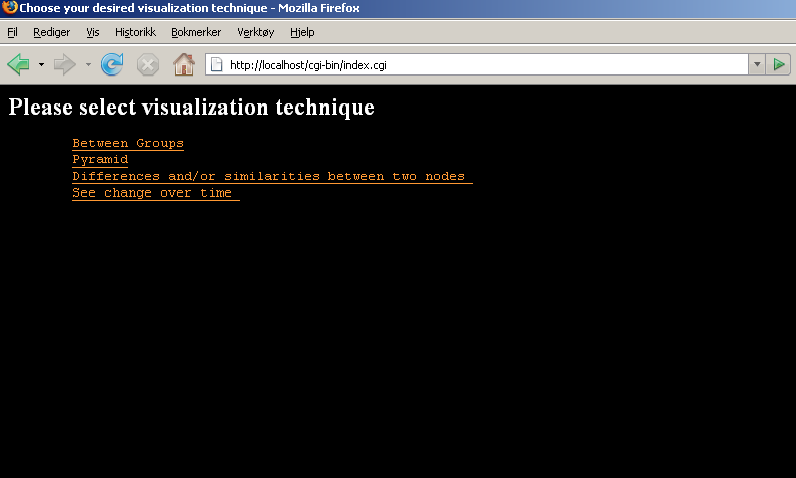
\includegraphics[scale=0.5]{screendumps/01_index.PNG} 
\caption{Start page} \label{um1}
\end{figure}
\newpage
From the menu, choose a visualization technique.(See \ref{techniques} for a discussion about the visualization types).In this example we choose `between groups'. On the next page, select how many criterias to visualize. (Between groups only). Click the submit button to continue.
%\begin{figure}[ht]
%\centering
%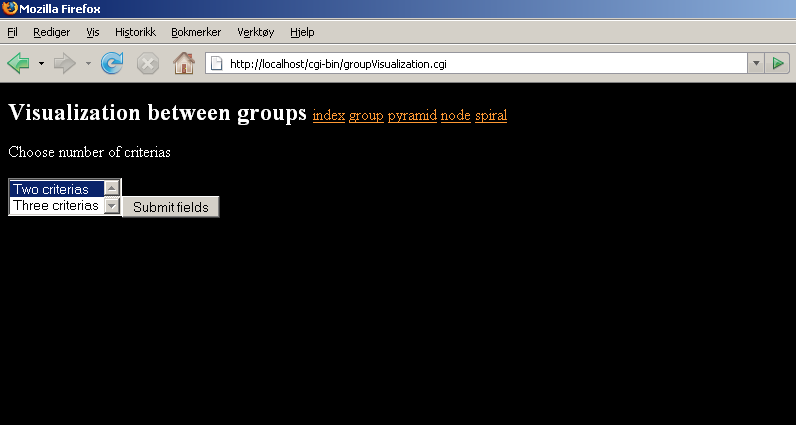
\includegraphics[scale=0.5]{screendumps/02_between_groups.PNG} 
%\caption{Start page} \label{um2}
%\end{figure}

From the drop down lists, select the components you want, then press the submit button.
\begin{figure}[hb]
\centering
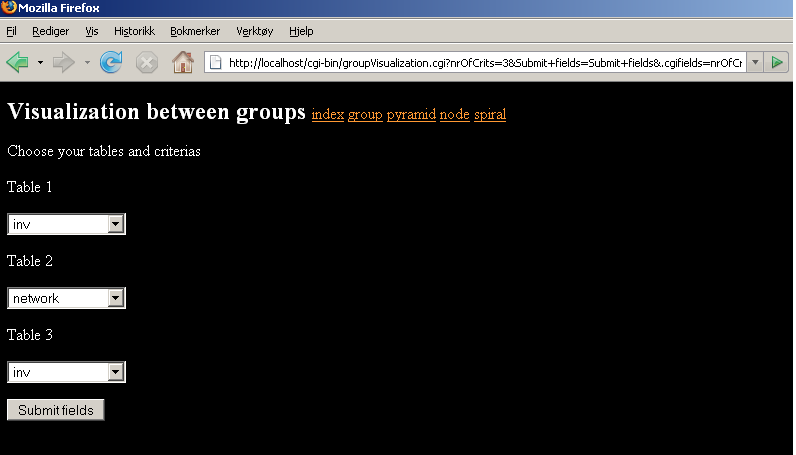
\includegraphics[scale=0.5]{screendumps/03_choose_tables.PNG} 
\caption{Select components} \label{um2}
\end{figure}

\newpage

Choose the desired fields. In this example, we will be generating a visualization based on Operating System, gateway, and emphasize the nodes with owner field set to Informatics. 


\begin{figure}[ht]
\centering
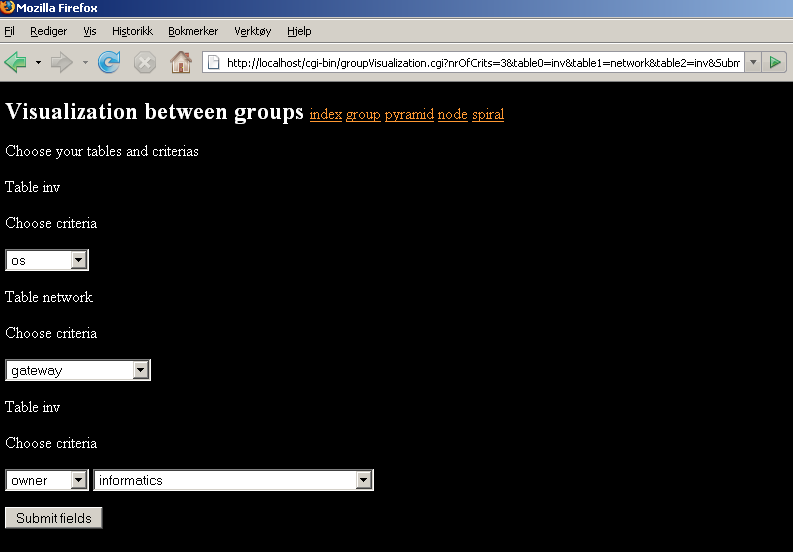
\includegraphics[scale=0.5]{screendumps/04_choose_values.PNG} 
\caption{Select values} \label{um4}
\end{figure}

Click the submit button to start generating the visualization.
\paragraph{Notice!}
In some rare cases, where imported fields don't have any values set in the XML files, the select boxes are empty. If an empty value is selected, an error message will be produced, in which case you must go back and select a different value or table.

\newpage
The visualization will be embedded in the browser window. You could also click the fullscreen link to open the file in the standalone Octaga Player. To choose different fields or visualizations, use the menu links on top of the page.
\paragraph{Notice!}
On some systems, after generating several different visualizations, the embedded VRML file will not be updated. We believe this is a browser problem. A work-around is to either close the browser completely and restart it, or opening the files in fullscreen mode with the link on the top of the page.

\begin{figure}[ht]
\centering
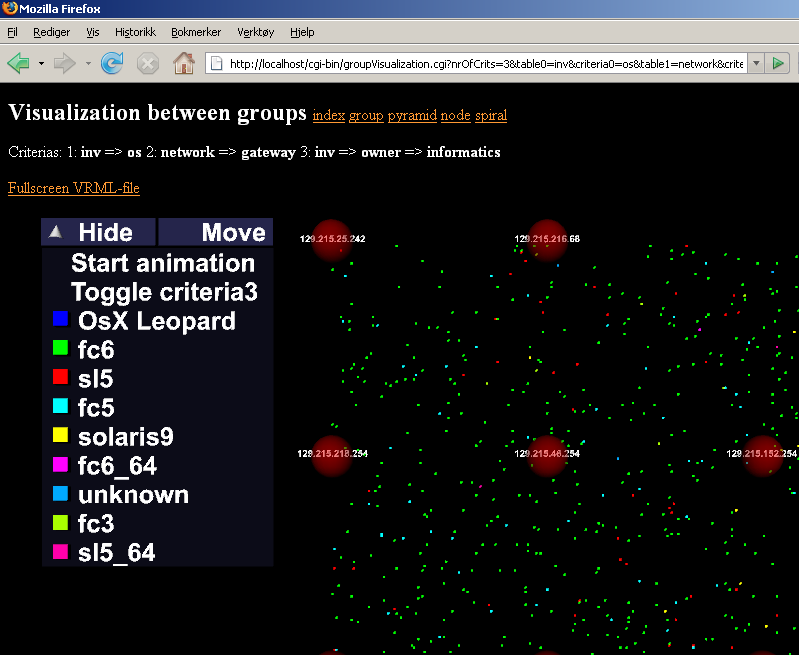
\includegraphics[scale=0.5]{screendumps/07_groupVis.PNG} 
\caption{Select components} \label{um5}
\end{figure}
 


\section{The visualizations}
\label{techniques}
All the visualizations are VRML code which follows the VRML97 specifications and are generated on-the-fly based upon the criteria given by the end user. The generated code has been tested and found to be working in Octaga Player.

You can navigate inside the VRML worlds by using either the arrow buttons on your keyboard or left-clicking the mouse and moving it. For more information about navigation in Octaga Player, refer to the `Octaga Player usermanual'. \footnote{http://www.octaga.com/freedownloads/OctagaPlayer/current/User\%20Manual.pdf}

Most of the techniques require the user to select one or more criteria from which the system generates clusters or groups.

\subsection{The HUD Menu}
The different visualizations all generate a HUD (Heads Up Display) menu with some common elements. 
The top bar of the menu consists of two elements: A `hide' field and a `move' field. The menu can be hidden by clicking on the hide field. Whilst hidden, another click will cause the menu to expand again.
The menu can be moved into a different position by clicking and holding the move field and dragging it to the desired position (drag and drop).The actual menu content may vary, depending on the visualization technique chosen. 

\subsection{Visualization between groups}
Criteria needed: Two or three\\
This visualization consists of all the individual nodes in the network along with  spheres representing the different groups derived from the second criteria. Every computer is shown as a cube, where the colour of the cube specifies its current value in the first criteria. When the user clicks `Start animation' on the HUD menu, the nodes will move to its belonging sphere group.
If used, the third criteria is a boolean true/false value, and the nodes fulfilling this criteria will be rotated around their own axis. To inspect a group, click the sphere and the viewpoint will zoom in to allow a closer look. Another click on the sphere will reset the viewpoint.
To filter different groups, click the HUD menu items you want to toggle. One click hides all the nodes in this group, and another one unhides. To inspect a single node, place the cursor over a node. The HUD menu will expand and reveal information about the selected node.
\paragraph{Notice!}
The node information displayed can be changed in the config file cfg/vscd.cfg, section `preferredfields'.
\subsection{Pyramid Visualization}
Criteria needed: Two\\

The pyramid visualization shows clusters as an hierarchial pyramid structure with maximum three steps. The first layer (red) shows all the nodes found in the database. The second layer shows the number of nodes fulfilling the first criteria, and the third layer shows the number of nodes fulfilling both first and second criteria. The HUD menu allows individual steps to be shown or hidden, and also allows the viewpoint to be changed. Additional information about a step is shown when the cursor is placed over the step.
\subsection{Node visualizer}
Criteria needed: Two\\

This technique compares two computers based upon their components.The visualization consists of two spheres (the nodes) and a grid of components. Arrows are drawn from the nodes to their belonging components and a component value shared by both nodes will be drawn in red.
One can inspect the dots connected to the components by placing the cursor over them, which triggers the key/value pair to be displayed in the HUD menu. One can also toggle the arrows belonging to one or both the nodes on and off by clicking the proper values in the HUD menu.

\subsection{Spiral}
Criteria needed: One.\\

This technique generates spheres for every unique value found in the criteria given. The sphere radius is decided by the number of nodes sharing the configuration. The result is shown as a spiral where the biggest clusters are placed in the middle. Each and every change in a single machine's configuration is shown as a slight colour change of the belonging sphere group. 
Depending on the amount of changes, the sphere colour is dark blue (no changes), lighter blue, green, yellow, red and purple (many changes). The HUD menu will show a calendar to track when the size and colours change, and the animation can be stopped and started again by pressing the play/stop buttons.


\chapter{System reference}

This part of the document contains documentation needed by developers for maintenance and expansion of the system. A more detailed System Reference is given in the LCFGVisualizers Complete Product Documentation,  and is currently only available in Norwegian. Documentation about specific methods and modules can be found in the program's source code which is commented in English.


\section{DataVisualizer}
The dataVisualizer is built as a three-layer program divided into GUI (Graphical User Interface), BLL (Business Layer Logic) and DAL (Data Access Layer). 
(For an illustration, see figure \ref{layers} in section \ref{app})
\subsection{GUI}
The GUI consists of the following files and classes: 
\subsubsection{cgiFunctions.pm}
Methods for printing HTML elements such as forms, stylesheets, menu, javascripts and embed visualizations.
Dependencies: DAL.pm

\subsubsection{cgi scripts}
\begin{itemize}
\item
Index.cgi -- Start page
\item
nodevisualization.cgi
\item
pyramidvisualization.cgi
\item
groupvisualization.cgi
\item
spiralvisualization.cgi
\end{itemize}
\begin{description}
\item[Dependencies:] CGI
\end{description}
\subsection{BLL}
The business layer.
\subsubsection{Visualization Library}
Consists of a library of visualization modules, namely:
\begin{itemize}
\item
GroupVisualizer
\item
PyramidVisualizer
\item
SpiralVisualizer
\item
NodeVisualizer
\end{itemize}

The visualizer modules depend on the following modules: 
\begin{description}
\item[Dependencies:]
DAL.pm, VRML\_Generator.pm
\end{description}

\subsection{VRML\_Generator}

The VRML\_Generator is the largest module and is used by all the visualization modules. Its main task is to generate valid VRML strings based on the attributes and method calls in the visualization modules. It is divided into different sections: 
\paragraph{Utility methods}
These are methods that can be used by any visualization, such as setting color values, generating vector positions, printing routes and converting strings to "VRML-safe" syntax.

\paragraph{General VRML methods}
These methods are also generic methods that generate valid VRML code from desired parameters. Many common VRML nodes can be generated, including `Timer', `Transform', `Group', `Interpolator' and `Text'. 
 
\paragraph{Proto methods}
Generates valid Proto nodes (static strings).
Proto nodes are definitions built by VRML nodes, fields and Scripts. Used to define MachineNodes, viewpoints and menuitems and their attributes.

\paragraph{Specific methods for each visualization technique}
This section contains methods used by only one specific visualization module.

\subsection{DAL}
The Data Access Layer. Connects to the database.
\begin{description}
\item[Files:] DAL.pm
\item[Dependencies:] DBI
\end{description}

\section{Bugs \& known issues}
\label{bug}

\subsection*{Web browser freezes/crashes}
On some systems, the octaga web browser plugin does not work.
\begin{description}
\item[Web browser:] Internet Explorer 7.0.5730.11
\item[Solution:] Change browser -- use firefox.
\item[Platform:] Systems running Windows XP SP2, Internet Explorer 7.0.5730.11, Octaga player 2.2.0.12
\end{description}

\subsection*{Octaga Player for Linux can not embed VRML}
This is expected to be fixed when Octaga releases Octaga Player 2.2 for Linux.

\subsection*{Octaga Player for Windows uses 100 \% CPU}
On some systems, Octaga uses a lot of resources.
This is often the case on a low-end computer, you might have better luck with a faster computer, lots of RAM and updated graphics card and -driver.

\subsection*{Embedded VRML in the web page is not updated}
When generating a visualization, the embedded file is sometimes not updated, and you will see an old file.
\paragraph{Solution:} Use the link on the top of the page to open the file in the standalone VRML viewer. This bug is probably related to the Octaga Browser plugin, it does not help to force reload or deleting Browser Cache. If you restart your web browser, the embedded file is updated.


\subsection*{Some links inside the VRML world do not work when using Cortona 3D viewer}
All links point to the same viewpoint. 
This is probably because anchors in the VRML file can have the same name.


\subsection*{TouchSensor is misplaced in VRML Player on Mac OSX}
When an object is linked with a touch sensor, one must click underneath the object to activate the sensor, rather than clicking the actual object. 

\subsection*{Empty fields from the database in the CGI}
When trying to visualize a field that has no values at all from the database, the select box in the web page is empty and it is impossible to draw a VRML file.
\paragraph{Solution:} Go back a few steps in the web page, and select another table.

\subsection*{Octaga Player for Linux can not show text nodes}
No text is shown in the Visualization. This bug is caused by Octaga Player being unable to find the system fonts. We have reported the bug to Octaga, and they have confirmed this to be an issue in version 2.1.


\section{Appendix}
\label{app}

\begin{figure}[ht]
\centering
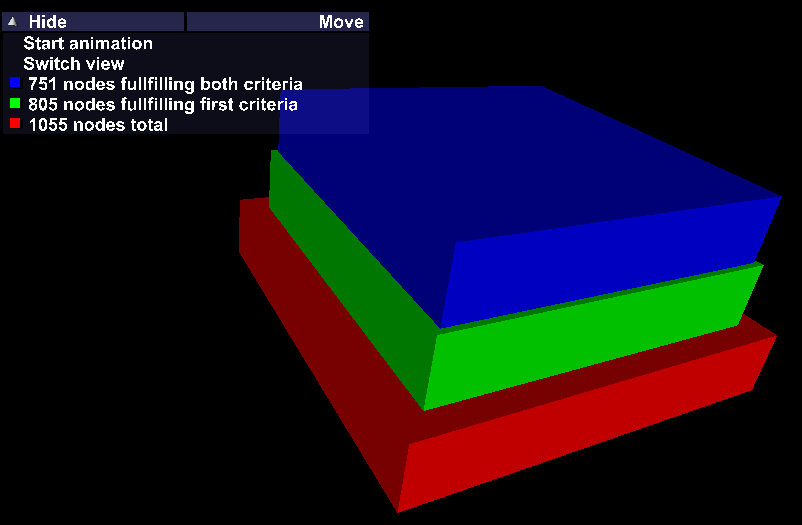
\includegraphics[scale=0.5]{pyramid2.PNG} 
\caption{Pyramid Visualization based on nodes with fc6 and owner informatics} \label{pyramid}
\end{figure}


\begin{figure}[hb]
\centering
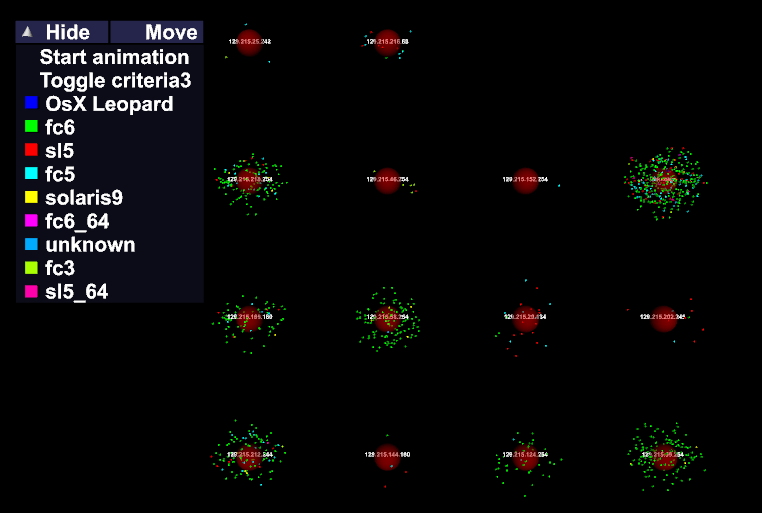
\includegraphics[scale=0.5]{06_groupVis.PNG} 
\caption{Group Visualization based on OS and gateway} \label{group}
\end{figure}


\begin{figure}[ht]
\centering
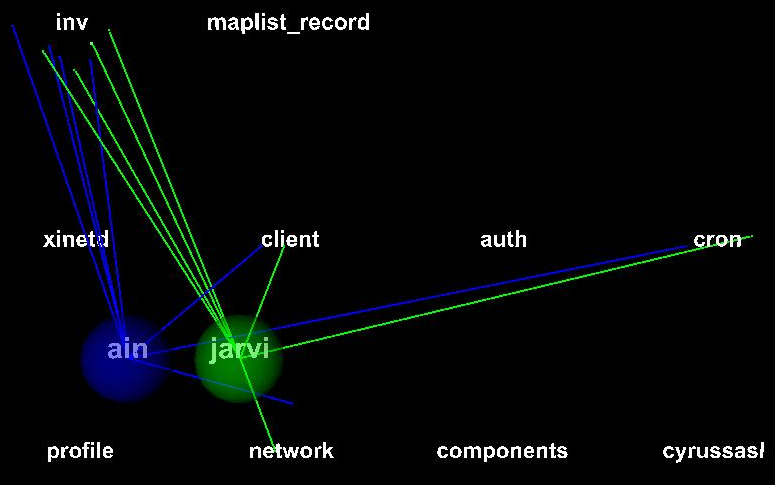
\includegraphics[scale=0.3]{nodevisudiffcompsainjarvi.png} 
\caption{Node Visualization showing different values} \label{nodes}
\end{figure}

\begin{figure}[ht]
\centering
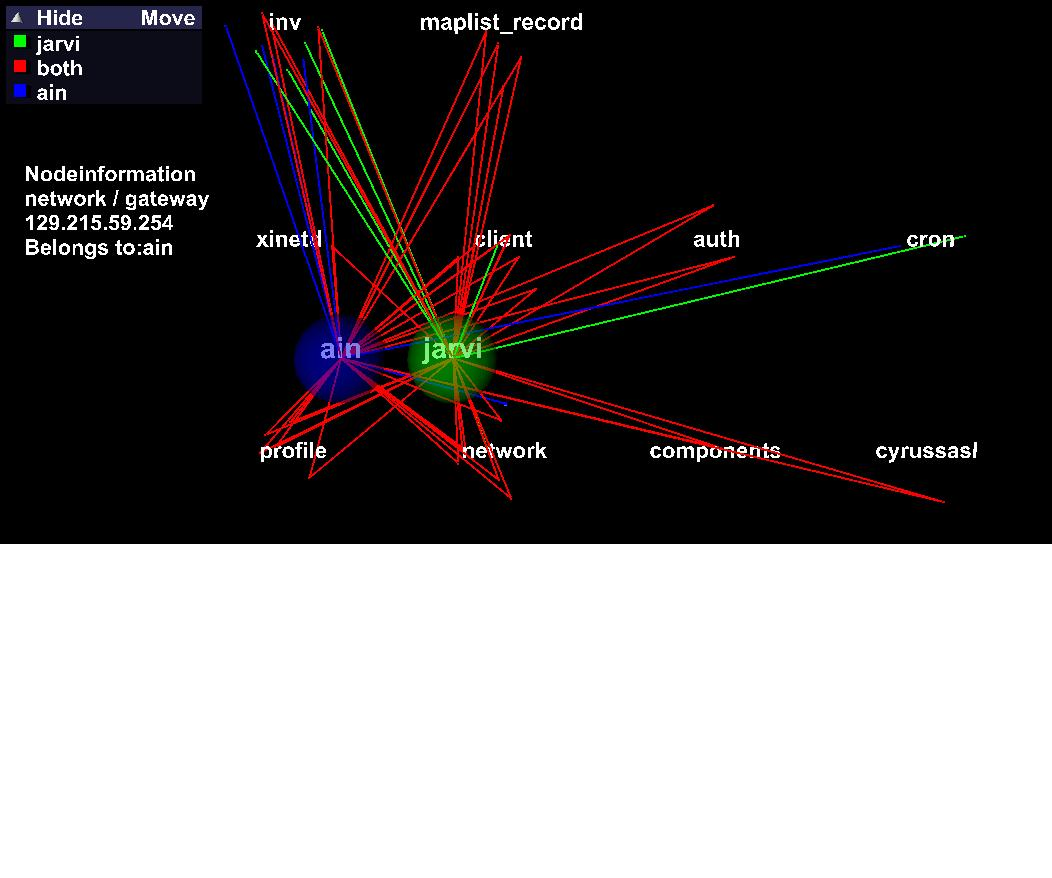
\includegraphics[scale=0.3]{nodevisuallcompsainjarvi.png} 
\caption{Node Visualization with both common and different values} \label{nodes}
\end{figure}

\begin{figure}[ht]
\centering
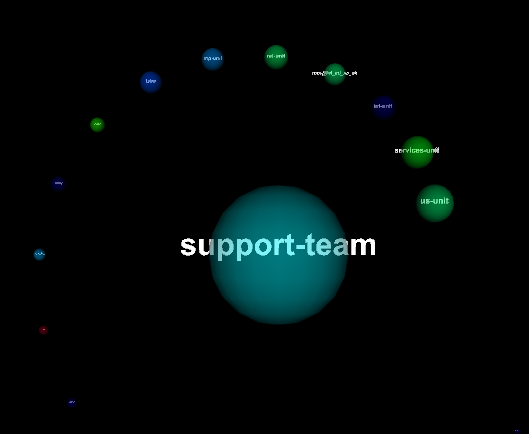
\includegraphics[scale=0.5]{spiral_manager.PNG} 
\caption{Spiral Visualization based on managers} \label{spiral}
\end{figure}

\begin{figure}[hb]
\centering
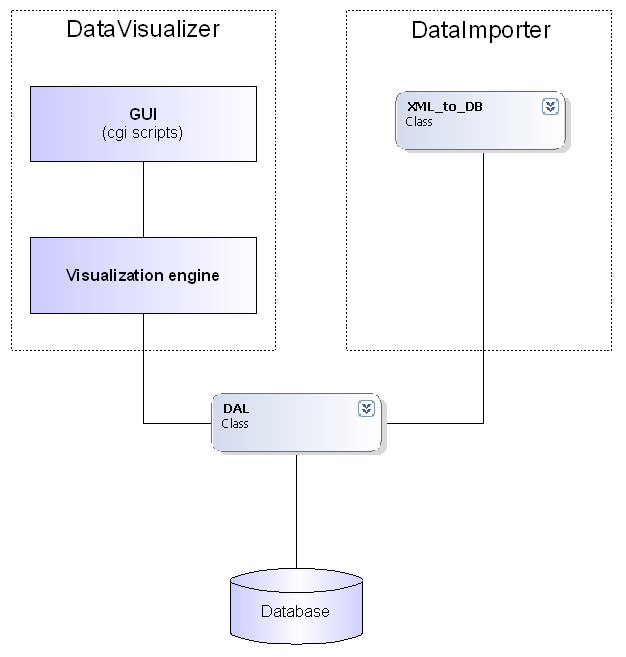
\includegraphics[scale=0.6]{Systemoversikt.png} 
\caption{System overview} \label{so}
\end{figure}
\newpage

\begin{figure}[hb]
\centering
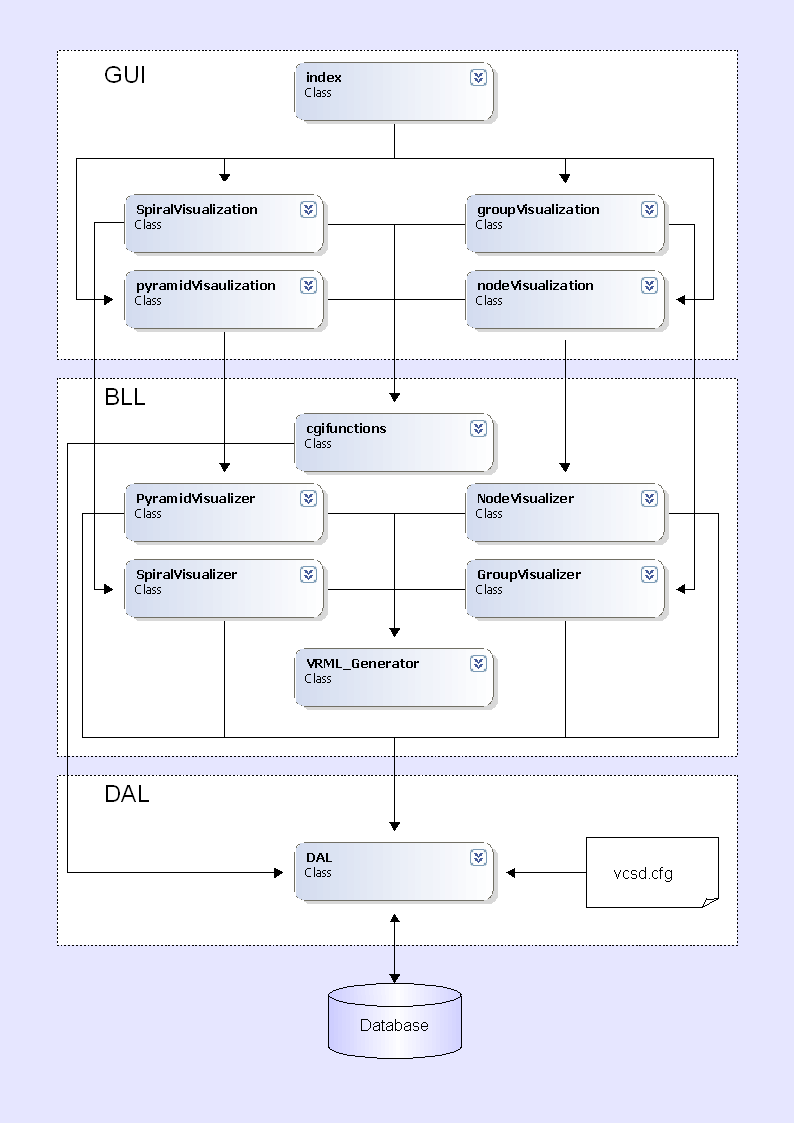
\includegraphics[scale=0.5]{DataVisualizerDetail.PNG} 
\caption{Structure} \label{layers}
\end{figure}



\end{document}
